\chapter{Analiza wymagań konkursu DAC SDC 2021}
\label{cha:Analiza probemu}

Opracowywany system powstaje na potrzeby konkursu \emph{Design Automation Conference System Design Contest 2021} (DAC SDC)
Rozpatrywanym problemem jest detekcja obiektów za pomocą sztucznej sieci neuronowej.
Realizacja zadania ma zostać przeprowadzona na wbudowanej platformie obliczeniowej typu \emph{SBC} (ang. \emph{Single Board Computer}) wyposażonej w~logikę rekonfigurowalną.
W~niniejszym rozdziale zostaną przedstawione założenia oraz wymagania stawiane wobec opracowywanego systemu detekcji, opisana docelowa platforma obliczeniowa, 
a także dostępne narzędzia wspomagające docelową implementację.


\section{Wymagania}
Opracowywany system powstaje na potrzeby konkursu, zatem rozwiązanie powinno spełniać stawiane założenia oraz wymagania dotyczące realizowanego zadania i~jego implementacji.
Zadaniem jest detekcja pojedynczych obiektów za pomocą sieci neuronowych na sekwencjach zarejestrowanych przez drona.
Organizatorzy dostarczają zbiór treningowy składający się z~obrazów o~wymiarach 640 pikseli szerokości na 360 pikseli wysokości. Zbiór składa się z~ponad 90 tysięcy obrazów, wchodzących w~skład 95 sekwencji podzielonych na 12 kategorii. Na rysunku \ref{fig:sample_images} przedstawiono przykładowe obrazy znajdujące się w~zbiorze uczącym wraz z~zaznaczonymi obiektami.
\begin{figure}
    \centering
    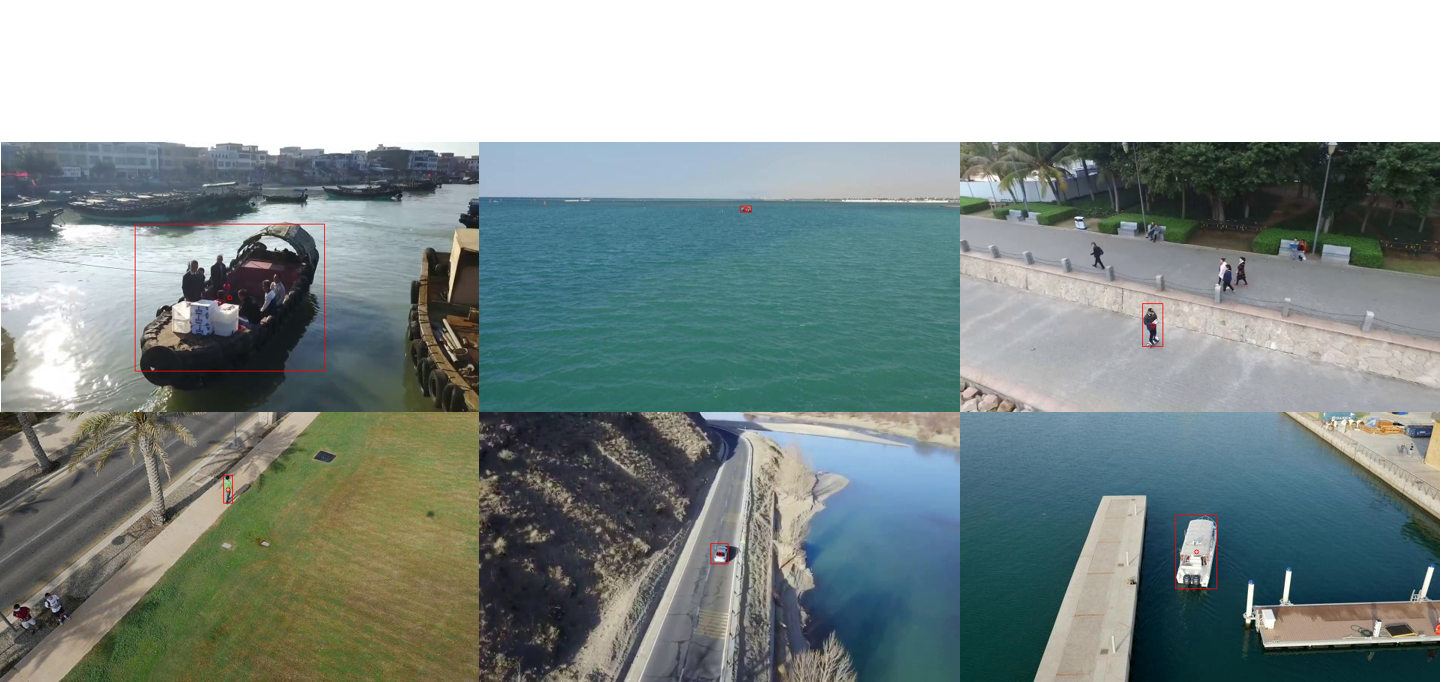
\includegraphics[width=\linewidth]{images/sample_images.png}
    \caption{Przykładowe obrazy zbioru uczącego wraz z~zaznaczonymi obiektami detekcji. Źródło \cite{dac_sdc_2021}.}
    \label{fig:sample_images}
\end{figure}

Samo rozwiązanie poddawane jest ocenie danej wzorem \eqref{eq:score}. Uzyskanie wyższej wartości skutkuje uzyskaniem wyższego miejsca w~rankingu, z~czego wynika, iż funkcję $Score$ należy maksymalizować. 

\begin{equation}
E_{Score} = log_2(E)
\label{eq:e_score}
\end{equation}
\begin{equation}
IoU_{Score} = max(0.1, ReLU(1 - 5 ReLU(0.7 - IoU)))
\label{eq:iou_score}
\end{equation}
\begin{equation}
FPS_{Score} = ReLU(1 - ReLU( 1 - \frac{FPS}{30}))
\label{eq:fps_score}
\end{equation}
\begin{equation}
Score = \frac{10^2}{E_{Score}} IoU_{Score} FPS_{Score}
\label{eq:score}
\end{equation}

Ocenie poddawana jest zarówno dokładność detekcji mierzona współczynnikiem $IoU$ (ang. \emph{Intersection over Union}), lecz również przepustowość $FPS$ mierzona poprzez liczbę przetworzonych obrazów na sekundę.
Sam współczynnik $IoU$ definiowany jest jako stosunek powierzchni (liczby pikseli) części wspólnej obszaru referencyjnego $X_{ref}$ oraz obszaru wyznaczonego $X_{pred}$ do łącznej powierzchni obu obszarów. Wyrażone to zostało za pomocą wzoru \eqref{eq:iou_eq}.
\begin{equation}
IoU = \frac{|X_{ref} \cap X_{pred}|}{|X_{ref} \cup X_{pred}|}
\label{eq:iou_eq}
\end{equation}
Ponadto mierzona jest również całkowita energia $E$ zużyta przez układ -- wyznaczana jako iloczynu czasu przetwarzania oraz średniej mocy układu (w czasie przetwarzania). 
Chwilowe wartości mocy są odczytywane z~regulatora mocy z~częstotliwością próbkowania $20 Hz$.
Zarówno pomiar energii oraz czasu musi być realizowany przez opracowaną aplikację.
Wstępna analiza pozwala stwierdzić, iż uzyskanie wartości $IoU$ oraz $FPS$ poniżej wartości progowych skutkuje zastosowanie kary, natomiast
%nadmierne 
zwiększanie tych wartość powyżej wartości progowych nie przynosi dodatkowych korzyści (przynajmniej w~sposób bezpośredni). 

% Analizując wzór \eqref{eq:fps_score} można zauważyć, iż uzyskanie przepustowości powyżej $30 fps$ pozwala na osiągnięcie maksymalnej wartości współczynnika $FPS_{Score}$. Dalsze zwiększenie przepustowości nie zwiększa wartości $FPS_{Score}$. 
% Dla deterministycznego systemu wartość ta powinna być stała. Oczekiwane jest również, iż dla różnych egzemplarzy platformy wartości te będą przyjmowały zbliżoną wartość. Wówczas Funkcja oceny \eqref{eq:score} zależy jedynie od dokładności oraz zużycia energii.

Wśród wymagań znajdują się również informacje odnośnie dostarczenia wymaganych plików.
Aplikacja sterująca ma być zrealizowana w~postaci notatnika \emph{Jupyter}.
Dodatkowo należy dostarczyć również pliki \emph{*.hwh} (plik opisu diagramu blokowego logiki programowalnej)
oraz \emph{*.bit} (plik konfiguracji logiki programowalnej) Ponadto należy dołączyć inne niezbędne do poprawnego działania aplikacji pliki. 
Finalne rozwiązanie musi być dostępne w~formie otwarto-źródłowej.

\section{Platforma sprzętowa}
Ewaluacja wytrenowanej sieci neuronowej jest przeprowadzana na platformie obliczeniowej \emph{Avnet Ultra96-V2} \cite{avnet_ultra96}. 
Jest to płytka rozwojowa wyposażona w~układ \emph{Xilinx Zynq UltraScale+ MPSoC ZU3EG A484}, 2 GB pamięci LPDDR4, slot kart microSD, moduł Wi-Fi, a~także porty USB 3.0, porty IO oraz port mini-display. 
Układ działa pod kontrolą systemu operacyjnego \emph{PetaLinux} wraz z~uruchomionym serwerem \emph{Jupyter} (pochodzących z~dystrybucji projektu \emph{Pynq}\cite{pynq}). 
Sam układ \emph{Xilinx Zynq UltraScale+ MPSoC ZU3EG A484} jest układem typu SoC. 
Zawiera czterordzeniowy procesor ARM Cortex-A53 MPCore, dwurdzeniowy procesor Arm Cortex-R5F MPCore oraz procesor graficzny Mali-400 MP2 \cite{zynq_product_guide}. 
Ponadto układ wyposażony jest w~logikę programowalną połączoną z~systemem procesorowym magistralą AXI. 
Logika programowalna zawiera: 
154 tys. \emph{System Logic Cells} (\emph{SLC}), 
141 tys. przerzutników (ang. \emph{Flip-Flops}, \emph{FF}) 
oraz 71 tys. \emph{LUT} (ang. Look-Up Table) zawartych w~blokach \emph{CLB} (ang. \emph{Configurable Logic Block}), 360 \emph{DSP slice}, 1.8 MB pamięci \emph{distributed RAM}, a~także 7.6 MB pamięci zawartej w~216 blokach \emph{BRAM}. 

\emph{SLC} jest to miara określająca możliwości czy liczbę zasobów umożliwiającą porównanie układów logiki programowalnej.
Jeden \emph{SLC} stanowi 1 \emph{LUT} pozwalający na realizację 6-o elementowej funkcji logicznej, 2 przerzutniki oraz dodatkowe elementy logiczne t.j. multiplekser. 

Bloki \emph{CLB} \cite{clb} dzielą się na dwa typy:
\begin{description}
\item \emph{SLICEL} -- jest zbudowany z 8 \emph{LUT}, 16 przerzutników, 8-bitowego łańcucha przeniesień (ang. \emph{carry chain}) oraz 7 multiplekserów. 
Elementy \emph{LUT} możliwe są do konfiguracji pozwalającej na realizację dowolnej funkcji logicznej o~7-u, 8-u lub 9-u wejściach lub wybranych funkcji o~55-u wejściach. 
Uzyskane rezultaty mogą zostać zapamiętane w~pamięci przerzutników (FF -- ang. \textit{Flip Flop}).
\item \emph{SLICEM} -- stanowi rozbudowany \emph{SLICEL} o~dodatkowe elementy pamięci możliwe do konfiguracji w~postaci 64 bitowej pamięci \emph{Distributed RAM} lub 32 bitowego rejestru przesuwnego. 
\end{description}

\emph{DSP} (ang. \emph{Digital Signal Processor}) \cite{dsp} stanowią elementy obliczeniowe pozwalające na realizację, operacji arytmetycznych czy logicznych.
Charakteryzują się niewielkim zużyciem energii oraz dużą elastycznością.
Możliwe są konfiguracje m.in. jako sumator, mnożarka czy nawet akumulator iloczynów sygnałów wejściowych.

Blok \emph{BRAM} (ang. \emph{Block RAM}) \cite{bram} stanowi 36Kbit pamięci o~2 portach do zapisu i~2 portach do odczyt. 
Możliwa jest konfiguracja jako 2~niezależne pamięci do 18Kbit, a~także jako kolejka \emph{FIFO}.
Dodatkowo dostępny jest tryb uśpienia pamięci pozwalając na dynamiczne zarządzanie mocą. 

Rysunek \ref{fig:ultra96} przedstawia platformę docelową.

\begin{figure}
    \centering
    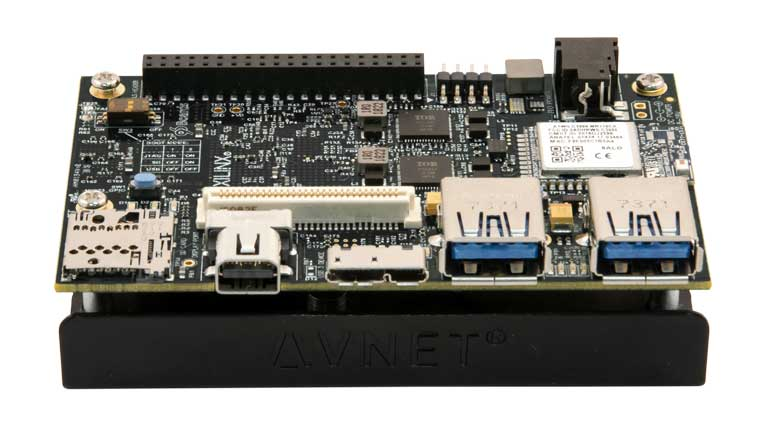
\includegraphics[width=\linewidth]{images/ultra96v2.png}
    \caption{Płytka \emph{Avnet Ultra96 V2}. Źródło \cite{avnet_ultra96}.}
    \label{fig:ultra96}
\end{figure}

\section{Narzędzia}
\label{ch:tools}
Uzyskanie przepustowości $30 fps$, pozwalającej na osiągnięcie wysokiej oceny rozwiązania, może być trudne lub niemożliwe  przy użyciu jedynie części procesorowej nawet dla modeli o~niskiej złożoności obliczeniowej. 
Wymagana jest tutaj dodatkowa akceleracja wykorzystująca logikę programowalną. 
W tym celu możliwe jest wykorzystanie istniejących narzędzi wspomagających sprzętową implementację sieci neuronowych, a~także procesu ich uczenia. 

Uczenie sieci z~przeznaczeniem do sprzętowej akceleracji zazwyczaj wiąże się z~wytrenowaniem modelu zmiennoprzecinkowego, następnie poddaniu go kwantyzacji oraz finalnie implementacji sprzętowej.
Etap wytrenowania modelu zmiennoprzecinkowego może zostać przeprowadzony z~użyciem
dowolnych narzędzi.
Korzystając z~formatu nie wspieranego wymagana może być zmiana reprezentacji.
Następnym etapem jest kwantyzacja wag oraz wyników pośrednich sieci, gdzie następuje przybliżenie liczb zmiennoprzecinkowych liczbami stałoprzecinkowymi lub binarnymi. 
Zazwyczaj wyniki sieci kwantyzowanej różnią się od wyników modelu zmiennoprzecinkowego, przez co wymagane jest wznowienie procesu uczenia.
Istnieje też możliwość pominięcia początkowego treningu modelu zmiennoprzecinkowego.
Model kwantyzowany możliwy jest do sprzętowej implementacji z~wykorzystaniem wybranych narzędzi.

Poniżej wymieniono wybrane narzędzia wspomagające sprzętową implementację sieci neuronowych
\begin{itemize}
    \item \emph{Brevitas}\cite{brevitas} -- biblioteka dla framework'a \emph{PyTorch} \cite{pytorch}, przeznaczona do wspomagania kwantyzacji i~treningu QNN, rozwijana przez \emph{Xilinx}. Umożliwia trenowanie modeli kwantyzowanych, zmiennoprzecinkowych oraz mieszanych. Proces kwantyzacji wymaga zbudowania modelu z~predefiniowanych warstw przystosowanych do kwantyzacji. 
    Metoda kwantyzacji jest podawana jako parametr inicjalizacyjny, za pośrednictwem nazwy klasy \emph{kwantyzatora} -- predefiniowanej lub własnej implementacji. 
    Pozwala to na zastosowanie dowolnej techniki kwantyzacji, czyniąc narzędzie bardzo wygodnym -- w~szczególności w~środowisku naukowym.
    
    \item \emph{FINN}\cite{finn} -- framework rozwijany przez \emph{Xilinx} pozwalający na implementację sprzętową QNN w~architekturze przetwarzania potokowego. 
    Wymaga użycia modelu kwantyzowanego w~formacie \emph{ONNX} (ang. \emph{Open Neural Network Exchange}) uzyskanego np. z~\emph{Brevitas}.
    Narzędzie dokonuje implementacji za pośrednictwem \emph{HLS}. Oprócz opisu sprzętowego generowana jest również część programowa pozwalająca na sterowanie procesem akceleracji. 
    W~pewnym stopniu możliwe jest również uproszczenie modelu np. łącząc kolejne operacje z~użyciem stałych. 
    
    
    \item \emph{QKeras}\cite{qkeras} -- biblioteka dla framework'a \emph{TensorFlow}\cite{tf} pozwalająca na kwantyzację i~trening QNN. Narzędzie mniej elastyczne niż \emph{Brevitas}, lecz posiadające prosty i~przejrzysty interfejs. 
    Możliwa jest również automatyczna konwersja modelu zmiennoprzecinkowego do modelu zapisanego z~użyciem kwantyzowanych odpowiedników.
    
    \item \emph{hls4ml}\cite{hls4ml} -- biblioteka dokonująca konwersji modelu QNN (\emph{QKeras}) do zapisu z~użyciem języka HLS.
    Posiada prosty interfejs. 
    Możliwe jest m.in. ustawienie parametrów ponownego użycia zasobów, czy optymalizacja wybranych elementów modelu. 
    
    \item \emph{Vitis AI}\cite{vitis_ai} -- środowisko pozwalające na przeprowadzenie kwantyzacji, optymalizacji architektury sieci oraz sterowania procesem akceleracji poprzez stosowne biblioteki C++/Python. Jest to środowisko rozwijane przez firmę \emph{Xilinx}.
    Wykorzystywana jest tutaj akceleracja z~wykorzystaniem generycznego, konfigurowalnego koprocesora DPU (ang.\textit{ Deep Processing Unit)}. 
    
\end{itemize}


Na etapie analizy problemu uwzględniono zarówno wymagania konkursowe, dostępną platformę sprzętową, a~także  narzędzia wspomagające sprzętową implementację.
Głównym celem jest implementacja szybkiego i~energooszczędnego rozwiązania, pozwalającego na dokładną detekcję pojedynczych obiektów. 
Zadanie jest realizowane w~oparciu o~sprzętową akcelerację wykorzystującą logikę programowalną płytki \emph{Avnet Ultra96 V2}.
Dostępnych jest wiele narzędzi usprawniających proces kwantyzacji, jak również implementacji sprzętowej.
W edycji 2021 konkursu zmieniono w~stosunku do lat poprzednich funkcję oceny \eqref{eq:score}. Liniowa zależność zużycia energii została zastąpiona logarytmiczną \eqref{eq:e_score}. 
Zmniejszono wagę związaną z~przepustowością oraz dokładnością, a~także zastosowano dodatkową ``zewnętrzną'' funkcję $ReLU$. 
Ponadto funkcja oceny jakości \eqref{eq:iou_score} dla $iou < 0.52$ przyjmuje wartość $0.1$. 
W poprzednich edycjach dla $iou < 0.5$ funkcja ``zerowała'' ostateczna ocenę.   
Wymóg udostępnienia rozwiązania w~formie otwarto-źródłowej pozwala na przegląd rozwiązań z~edycji poprzedzających, a~tym samym na ich dalszy rozwój.

% Możliwe jest wykorzystanie lub wzorowanie się na istniejących już rozwiązaniach zapewniających wysoką przepustowość oraz niskie zużycie energii. 


% Należy zaznaczyć, iż architektury sieci przed i~po procesie kwantyzacji nie mogą lub nie powinny być rozważanie jako identyczne ze względu na znaczne zmiany jakie wprowadza kwantyzacja.  


%---------------------------------------------------------------------------

    

